\chapter{Witness Results and Failure Analysis}
\label{ch:witness-results-failure-analysis}

\section{The governing safety question}
The battery witness row answers one governing question for the dissertation: when
telemetry degrades, can a runtime layer reduce true-state safety loss without pretending
that nominal controller legality is enough? This chapter treats the battery row as the
deepest defended empirical surface because it closes the full ORIUS loop from degraded
observation, to repaired action, to governed release.

\section{Witness experiment design}
The witness experiments are not meant to show that ORIUS dominates every plant-specific
controller under every cost metric. They are designed to test a narrower and more important
claim: whether a certificate-aware runtime can keep hidden true-state violations from
passing through a nominally coherent observation surface. The baselines therefore include
controllers that are cheaper, controllers that are more aggressive, and controllers that
already include some robustness logic, because the scientific question is not merely who
optimizes best in nominal conditions. The question is what survives once the observation
channel itself begins to fail.

\section{Headline result}
The primary evidence surface is the main safety-and-cost table below.

\IfFileExists{paper/assets/tables/generated/tbl01_main_results.tex}{%
\begin{table}[htbp]
\centering
\scriptsize
\caption{Main safety and cost outcomes under telemetry faults.}
\label{tab:TBL01_MAIN_RESULTS}
\setlength{\tabcolsep}{4pt}
\renewcommand{\arraystretch}{0.96}
\resizebox{\linewidth}{!}{%
\begin{tabular}{lrrrrrrrrrr}
\toprule
controller & true\_soc\_violation\_rate\_mean & true\_soc\_violation\_rate\_ci\_low & true\_soc\_violation\_rate\_ci\_high & true\_soc\_violation\_severity\_p95\_mean & true\_soc\_violation\_severity\_p95\_ci\_low & true\_soc\_violation\_severity\_p95\_ci\_high & intervention\_rate\_mean & intervention\_rate\_ci\_low & intervention\_rate\_ci\_high & cost\_delta\_pct\_mean \\
\midrule
aci\_conformal & 0.000000 & 0.000000 & 0.000000 & 0.000000 & 0.000000 & 0.000000 & 0.020833 & 0.020833 & 0.020833 & 0.023244 \\
cvar\_interval & 0.191667 & 0.119427 & 0.274305 & 333.582626 & 0.265437 & 848.045446 & 0.000000 & 0.000000 & 0.000000 & -0.009092 \\
dc3s\_ftit & 0.000000 & 0.000000 & 0.000000 & 0.000000 & 0.000000 & 0.000000 & 0.088194 & 0.070139 & 0.105556 & 0.147639 \\
dc3s\_wrapped & 0.000000 & 0.000000 & 0.000000 & 0.000000 & 0.000000 & 0.000000 & 0.000000 & 0.000000 & 0.000000 & 0.054576 \\
deterministic\_lp & 0.129861 & 0.105555 & 0.170833 & 547.992608 & 198.317264 & 1056.208662 & 0.000000 & 0.000000 & 0.000000 & 0.000000 \\
robust\_fixed\_interval & 0.191667 & 0.119427 & 0.274305 & 333.582626 & 0.265437 & 848.045446 & 0.000000 & 0.000000 & 0.000000 & -0.009092 \\
scenario\_mpc & 0.000000 & 0.000000 & 0.000000 & 0.000000 & 0.000000 & 0.000000 & 0.000000 & 0.000000 & 0.000000 & 0.006481 \\
scenario\_robust & 0.000000 & 0.000000 & 0.000000 & 0.000000 & 0.000000 & 0.000000 & 0.000000 & 0.000000 & 0.000000 & 0.006481 \\
\bottomrule
\end{tabular}

}
\end{table}
%
}{%
\begin{table}[htbp]
\centering
\scriptsize
\caption{Main safety and cost outcomes under telemetry faults.}
\label{tab:TBL01_MAIN_RESULTS}
\setlength{\tabcolsep}{4pt}
\renewcommand{\arraystretch}{0.96}
\resizebox{\linewidth}{!}{%
\begin{tabular}{lrrrrrrrrrr}
\toprule
controller & true\_soc\_violation\_rate\_mean & true\_soc\_violation\_rate\_ci\_low & true\_soc\_violation\_rate\_ci\_high & true\_soc\_violation\_severity\_p95\_mean & true\_soc\_violation\_severity\_p95\_ci\_low & true\_soc\_violation\_severity\_p95\_ci\_high & intervention\_rate\_mean & intervention\_rate\_ci\_low & intervention\_rate\_ci\_high & cost\_delta\_pct\_mean \\
\midrule
aci\_conformal & 0.000000 & 0.000000 & 0.000000 & 0.000000 & 0.000000 & 0.000000 & 0.020833 & 0.020833 & 0.020833 & 0.023244 \\
cvar\_interval & 0.191667 & 0.119427 & 0.274305 & 333.582626 & 0.265437 & 848.045446 & 0.000000 & 0.000000 & 0.000000 & -0.009092 \\
dc3s\_ftit & 0.000000 & 0.000000 & 0.000000 & 0.000000 & 0.000000 & 0.000000 & 0.088194 & 0.070139 & 0.105556 & 0.147639 \\
dc3s\_wrapped & 0.000000 & 0.000000 & 0.000000 & 0.000000 & 0.000000 & 0.000000 & 0.000000 & 0.000000 & 0.000000 & 0.054576 \\
deterministic\_lp & 0.129861 & 0.105555 & 0.170833 & 547.992608 & 198.317264 & 1056.208662 & 0.000000 & 0.000000 & 0.000000 & 0.000000 \\
robust\_fixed\_interval & 0.191667 & 0.119427 & 0.274305 & 333.582626 & 0.265437 & 848.045446 & 0.000000 & 0.000000 & 0.000000 & -0.009092 \\
scenario\_mpc & 0.000000 & 0.000000 & 0.000000 & 0.000000 & 0.000000 & 0.000000 & 0.000000 & 0.000000 & 0.000000 & 0.006481 \\
scenario\_robust & 0.000000 & 0.000000 & 0.000000 & 0.000000 & 0.000000 & 0.000000 & 0.000000 & 0.000000 & 0.000000 & 0.006481 \\
\bottomrule
\end{tabular}

}
\end{table}
%
}

The table shows the core ORIUS result in the form that matters most for this dissertation.
Several plant-specific robust baselines already avoid true-state violations on this witness
task, so the contribution is not that ORIUS is the only safe controller in the table. The
contribution is that ORIUS closes the hidden-violation mode while keeping intervention,
repair, and certificate semantics explicit at runtime. In contrast, the deterministic and
interval baselines still exhibit material true-state violation rates once telemetry faults
are introduced, even though they remain internally well-posed optimization procedures.

That distinction is the witness-domain result. ORIUS is not claiming to replace every
robust controller with one universal optimizer. It is showing that a runtime layer can sit
between nominal control and physical release, detect when observation quality has changed
the meaning of legality, and then either repair the action or deny release under explicit
certificate semantics.

\section{Why the result happens}
The battery witness supports a mechanistic interpretation rather than a leaderboard reading.
ORIUS changes the release decision in three linked ways. Reliability loss is detected before
action release, uncertainty is widened before legality is checked, and unsafe actions are
either repaired or replaced before they reach the plant. The main table is therefore best
read as evidence that the release boundary changed, not simply as evidence that one model
forecasted more accurately than another.

\section{Ablation logic}
The ablation table shows where the runtime stack earns its gains and where those gains still
depend on the details of the degraded-observation regime.

\IfFileExists{paper/assets/tables/generated/tbl02_ablations.tex}{%
\begin{table}[htbp]
\centering
\footnotesize
\caption{Ablation study: DC$^3$S violation-rate reduction under telemetry faults. The gate requires both material effect ($\ge10$\% relative reduction) and statistical evidence ($p<0.01$); rows marked ``stat only'' improve significantly but miss the material-effect threshold.}
\label{tab:TBL02_ABLATIONS}
\setlength{\tabcolsep}{4pt}
\renewcommand{\arraystretch}{1.05}
\begin{tabularx}{\textwidth}{llrrrrX}
\toprule
Scope & Fault / baseline & $n$ & Base & DC$^3$S & Rel.\ red.\ (\%) & Gate \\
\midrule
primary & all & 160 & 0.250 & 0.231 & +7.7 & stat only; p=$<$0.001 \\
\midrule
secondary & delay+jitter & 40 & 0.253 & 0.230 & +9.3 & stat only; p=$<$0.001 \\
secondary & dropout & 40 & 0.250 & 0.226 & +9.7 & stat only; p=$<$0.001 \\
secondary & out-of-order & 40 & 0.252 & 0.230 & +8.9 & stat only; p=$<$0.001 \\
secondary & spikes & 40 & 0.250 & 0.231 & +7.5 & stat only; p=$<$0.001 \\
\midrule
sec.\ scenario & drift combo vs.\ deterministic LP & 10 & 0.350 & 0.300 & +14.3 & pass; p=0.002 \\
sec.\ scenario & drift combo vs.\ robust fixed & 10 & 0.250 & 0.300 & -20.1 & worse; p=0.002 \\
sec.\ scenario & dropout vs.\ deterministic LP & 10 & 0.350 & 0.300 & +14.3 & pass; p=0.002 \\
sec.\ scenario & dropout vs.\ robust fixed & 10 & 0.252 & 0.300 & -18.9 & worse; p=0.002 \\
\bottomrule
\end{tabularx}
\end{table}%
}{%
\begin{table}[htbp]
\centering
\footnotesize
\caption{Ablation study: DC$^3$S violation-rate reduction under telemetry faults. The gate requires both material effect ($\ge10$\% relative reduction) and statistical evidence ($p<0.01$); rows marked ``stat only'' improve significantly but miss the material-effect threshold.}
\label{tab:TBL02_ABLATIONS}
\setlength{\tabcolsep}{4pt}
\renewcommand{\arraystretch}{1.05}
\begin{tabularx}{\textwidth}{llrrrrX}
\toprule
Scope & Fault / baseline & $n$ & Base & DC$^3$S & Rel.\ red.\ (\%) & Gate \\
\midrule
primary & all & 160 & 0.250 & 0.231 & +7.7 & stat only; p=$<$0.001 \\
\midrule
secondary & delay+jitter & 40 & 0.253 & 0.230 & +9.3 & stat only; p=$<$0.001 \\
secondary & dropout & 40 & 0.250 & 0.226 & +9.7 & stat only; p=$<$0.001 \\
secondary & out-of-order & 40 & 0.252 & 0.230 & +8.9 & stat only; p=$<$0.001 \\
secondary & spikes & 40 & 0.250 & 0.231 & +7.5 & stat only; p=$<$0.001 \\
\midrule
sec.\ scenario & drift combo vs.\ deterministic LP & 10 & 0.350 & 0.300 & +14.3 & pass; p=0.002 \\
sec.\ scenario & drift combo vs.\ robust fixed & 10 & 0.250 & 0.300 & -20.1 & worse; p=0.002 \\
sec.\ scenario & dropout vs.\ deterministic LP & 10 & 0.350 & 0.300 & +14.3 & pass; p=0.002 \\
sec.\ scenario & dropout vs.\ robust fixed & 10 & 0.252 & 0.300 & -18.9 & worse; p=0.002 \\
\bottomrule
\end{tabularx}
\end{table}%
}

Some secondary scenarios clear the strict gate and others do not. That pattern matters
scientifically because it shows where the kernel is buying safety: not through a single
magic margin, but through a coupling between reliability estimation, uncertainty widening,
and local repair geometry. The ablations therefore support a sharper claim than simple
average improvement: ORIUS behaves like a genuine degraded-observation runtime layer whose
effect depends on the structure of the fault family.

\section{Coverage under reliability slices}
ORIUS depends on reliability-conditioned uncertainty rather than on a single fixed interval.
The grouped coverage table below is included to show why that distinction matters.

\IfFileExists{paper/assets/tables/generated/tbl03_cqr_group_coverage.tex}{%
\begin{table}[htbp]
\centering
\small
\caption{Regime-group CQR coverage and interval width summary.}
\label{tab:TBL03_CQR_GROUP_COVERAGE}
\begin{tabular}{llrrr}
\toprule
target & group & picp\_90 & mean\_width & sample\_count \\
\midrule
load\_mw & low & 0.852381 & 1244.838584 & 840 \\
load\_mw & mid & 0.883333 & 937.421883 & 840 \\
load\_mw & high & 0.910714 & 1028.215886 & 840 \\
wind\_mw & low & 0.976190 & 719.719141 & 840 \\
wind\_mw & mid & 0.934524 & 811.954083 & 840 \\
wind\_mw & high & 0.900000 & 969.921806 & 840 \\
solar\_mw & low & 0.802381 & 891.551155 & 840 \\
solar\_mw & mid & 0.822485 & 1016.613362 & 845 \\
solar\_mw & high & 0.737725 & 1206.156144 & 835 \\
\bottomrule
\end{tabular}

\end{table}
%
}{%
\begin{table}[htbp]
\centering
\small
\caption{Regime-group CQR coverage and interval width summary.}
\label{tab:TBL03_CQR_GROUP_COVERAGE}
\begin{tabular}{llrrr}
\toprule
target & group & picp\_90 & mean\_width & sample\_count \\
\midrule
load\_mw & low & 0.852381 & 1244.838584 & 840 \\
load\_mw & mid & 0.883333 & 937.421883 & 840 \\
load\_mw & high & 0.910714 & 1028.215886 & 840 \\
wind\_mw & low & 0.976190 & 719.719141 & 840 \\
wind\_mw & mid & 0.934524 & 811.954083 & 840 \\
wind\_mw & high & 0.900000 & 969.921806 & 840 \\
solar\_mw & low & 0.802381 & 891.551155 & 840 \\
solar\_mw & mid & 0.822485 & 1016.613362 & 845 \\
solar\_mw & high & 0.737725 & 1206.156144 & 835 \\
\bottomrule
\end{tabular}

\end{table}
%
}

Coverage quality moves materially across regimes, especially in the harder operating slices.
That is exactly the pattern ORIUS is designed to take seriously. If interval behavior were
uniform, a fixed robust margin would be closer to sufficient. Because interval behavior
changes with regime and reliability, the runtime needs to tighten admissible action as trust
in the observation surface falls.

\section{Bounded novelty inside the witness row}
The witness row also contains a bounded learned-reliability novelty surface. It matters
here only insofar as it improves the degraded-observation safety argument rather than
turning the dissertation into a forecasting paper.

\begin{figure}[htbp]
\centering
\IfFileExists{reports/publication/fig_battery_deep_oqe_safety_metrics.png}{%
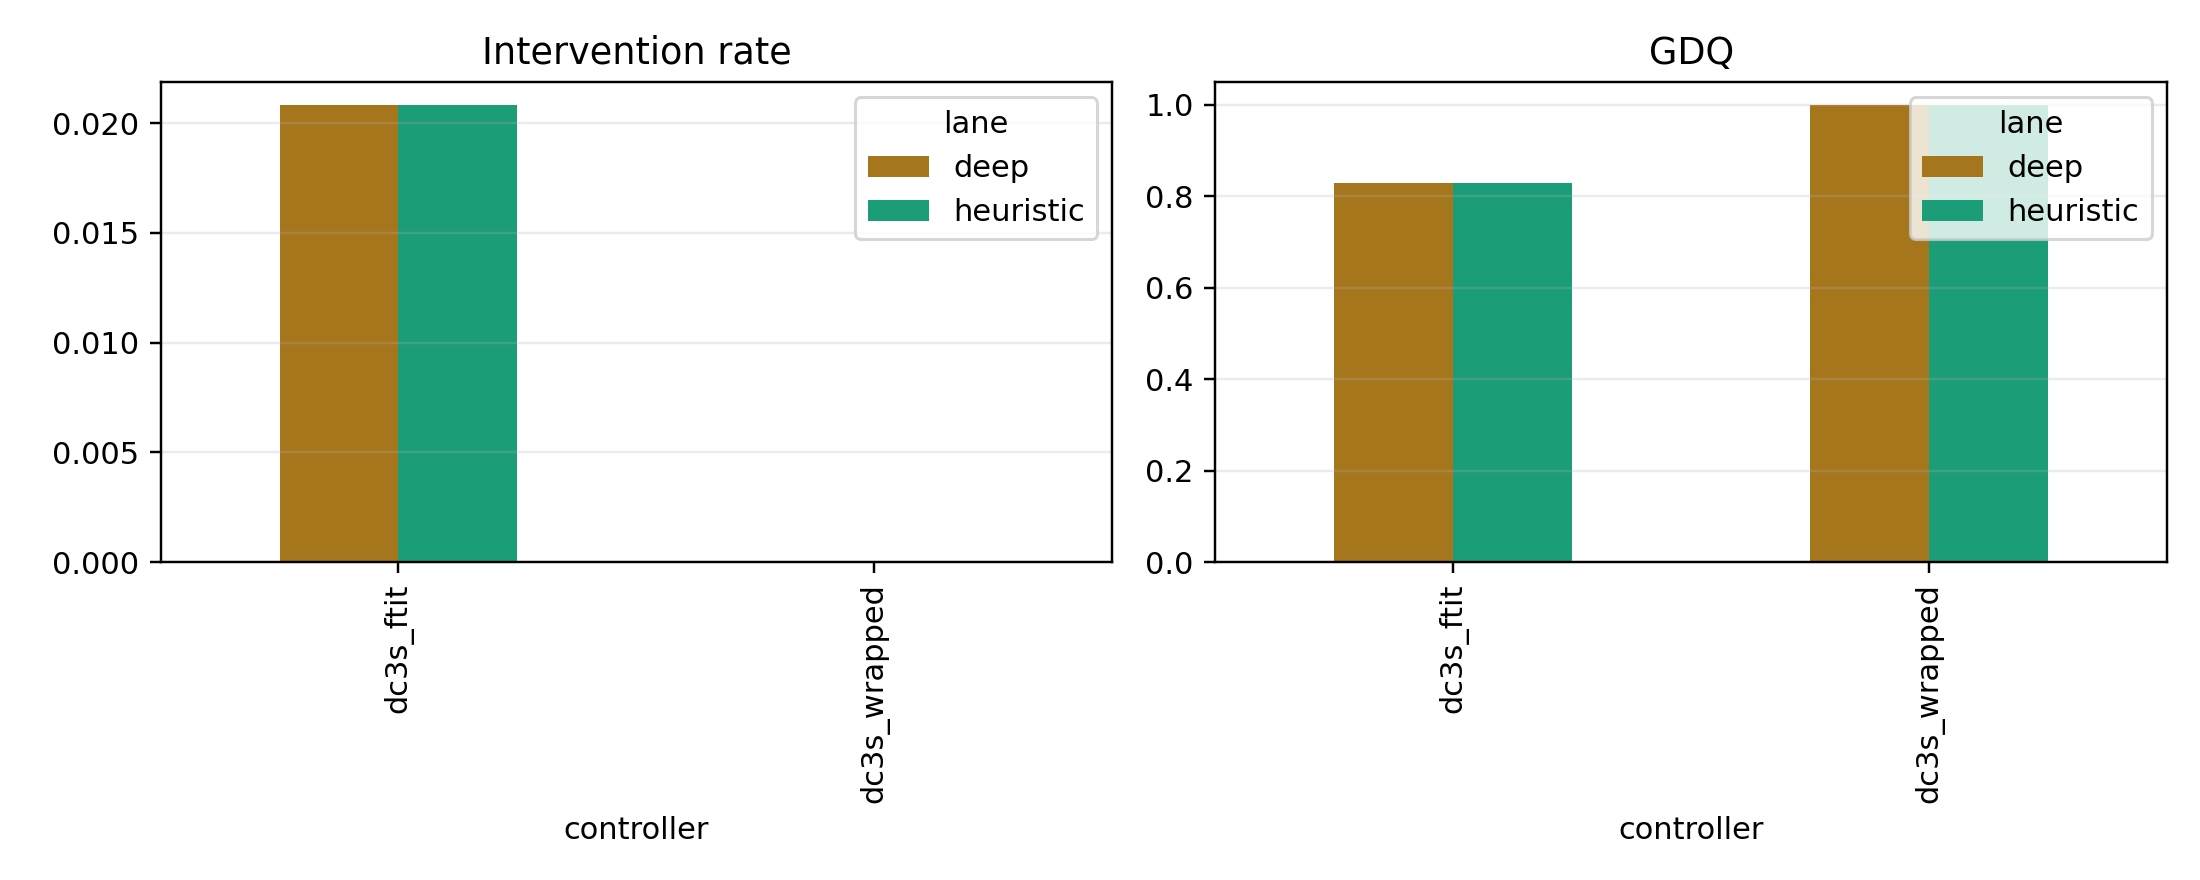
\includegraphics[width=0.82\textwidth]{reports/publication/fig_battery_deep_oqe_safety_metrics.png}%
}{%
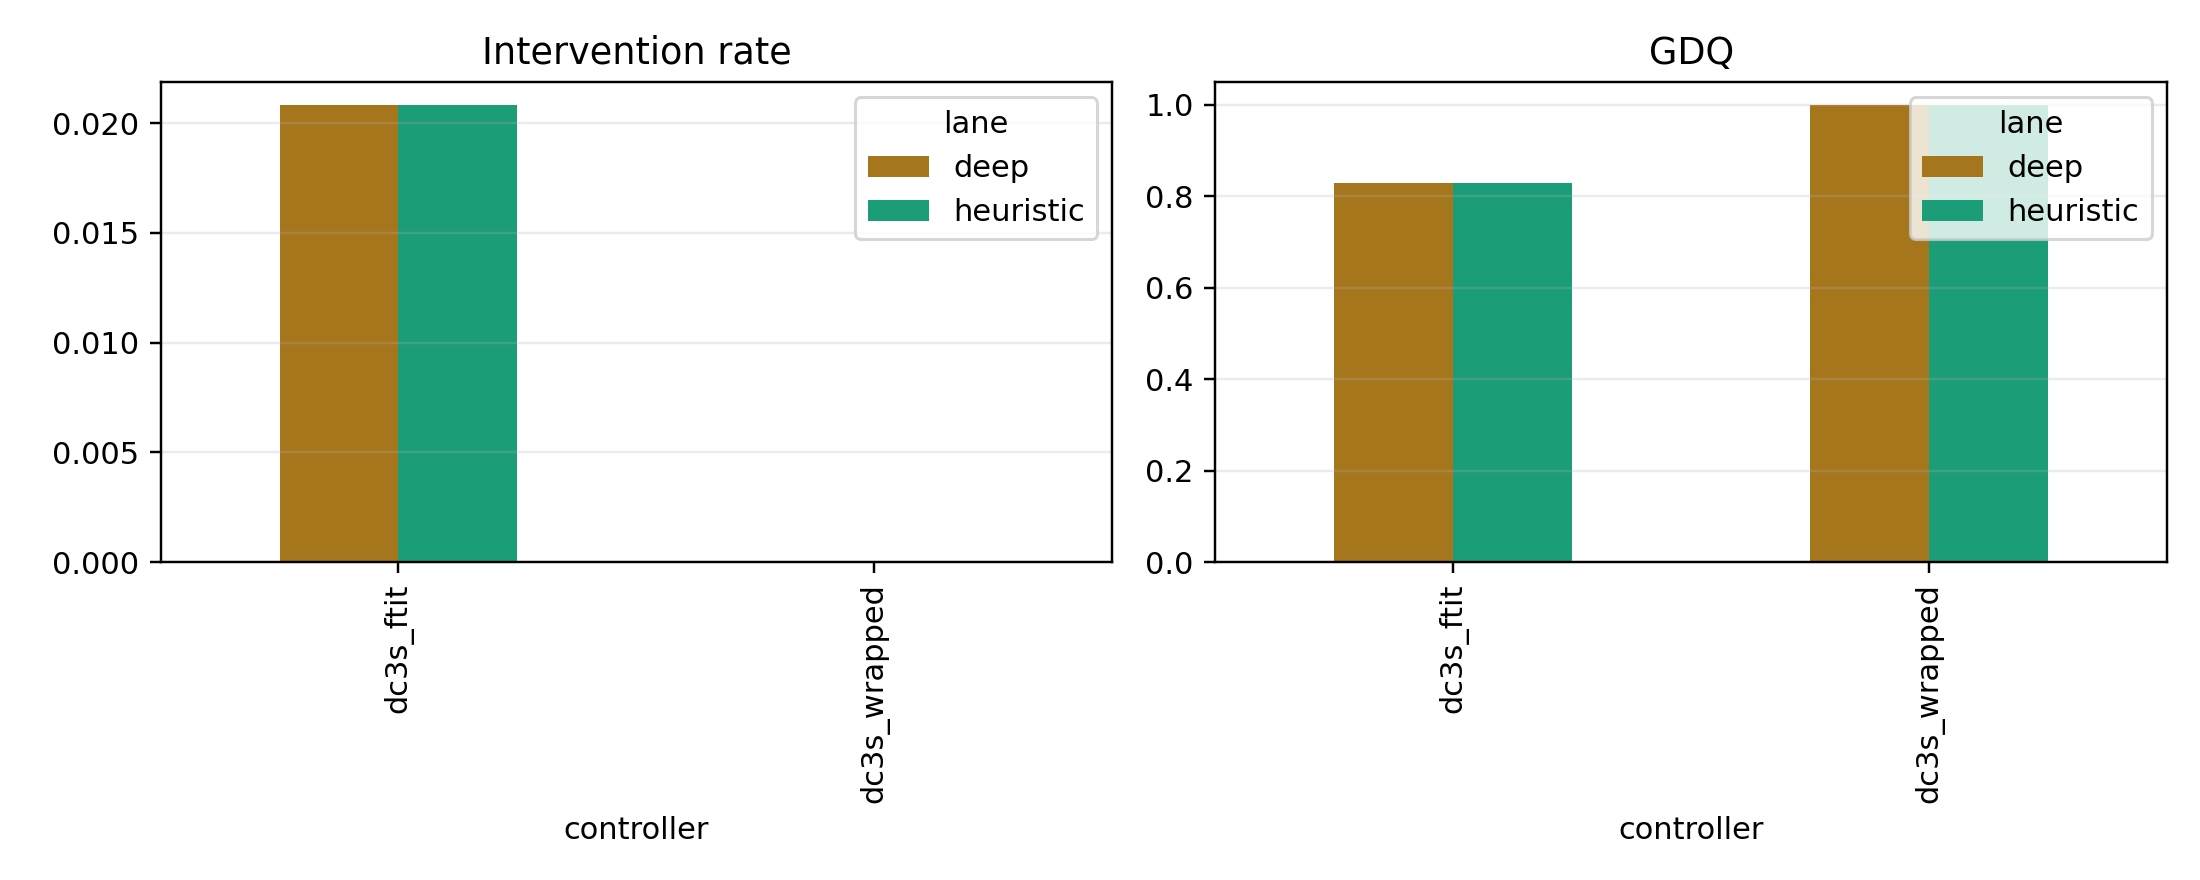
\includegraphics[width=0.82\textwidth]{../reports/publication/fig_battery_deep_oqe_safety_metrics.png}%
}
\caption{Battery learned-reliability safety surface. The deep model is judged by
true-state safety, intervention burden, and certificate-valid release behavior rather than
by forecast error alone.}
\label{fig:battery-deep-oqe-safety}
\end{figure}

The figure supports a narrower point than the main safety table. It shows that the learned
reliability path can improve the runtime's discrimination of when to intervene and when to
allow nominal action to pass. That is a bounded novelty claim about the observation side of
ORIUS, not a replacement for the main witness claim about repaired release under degraded
telemetry.

\section{Without ORIUS}
Without ORIUS, the telemetry fault is treated as a nuisance external to the release
decision. The deterministic and interval baselines in the headline table expose exactly what
goes wrong under that assumption: the controller remains computationally coherent while
true-state violation reappears. Without calibrated widening, the controller checks legality
against the wrong state set. Without repair, the unsafe action is still released. Without
certificate discipline, the runtime cannot later explain why the action was allowed or when
fallback should have taken over.

\section{What still remains bounded}
The battery chapter therefore supports three distinct claims. First, it supports a strong
witness claim that ORIUS can materially improve degraded-observation safety on a defended
row. Second, it supports a bounded robustness claim that the kernel remains meaningful across
multiple telemetry fault families rather than on one curated failure. Third, it supports a
runtime-governance claim that intervention and certificate behavior are part of the result,
not merely surrounding instrumentation. Deeper learned-reliability artifacts remain in the
governed package, but the main witness conclusion is already visible here: once legality on
the observed state is no longer enough, ORIUS changes the release boundary in a measurable
and auditable way.
